
%----------------------------------------------------------------------------------------
%	Lecture 12
%----------------------------------------------------------------------------------------

\chapter{Definite Integrals}
\bigbreak

\section{Area under a curve}

\begin{enumerate}
	\item Divide region into rectangles.
	\item Add up area of rectangles.
	\item Take limit as rectangles become thin.
\end{enumerate}


\begin{figure}[ht!]
	\centering
	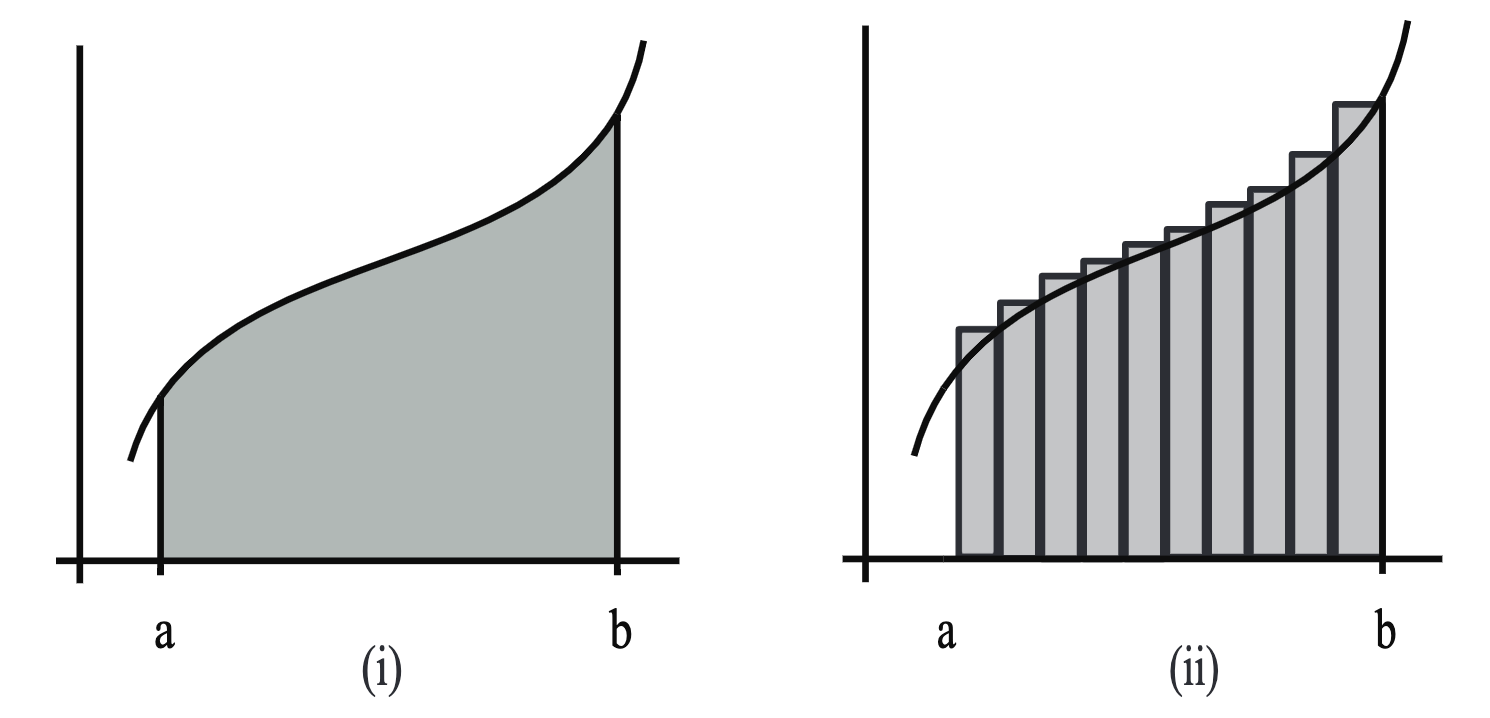
\includegraphics[scale=0.5]{./images/lecture_12_figure_1.png}
	\caption{(i) Area under the curve; (ii) sum of areas under the rectangles}
\end{figure}


\subsection{General Picture}

\begin{figure}[ht!]
	\centering
	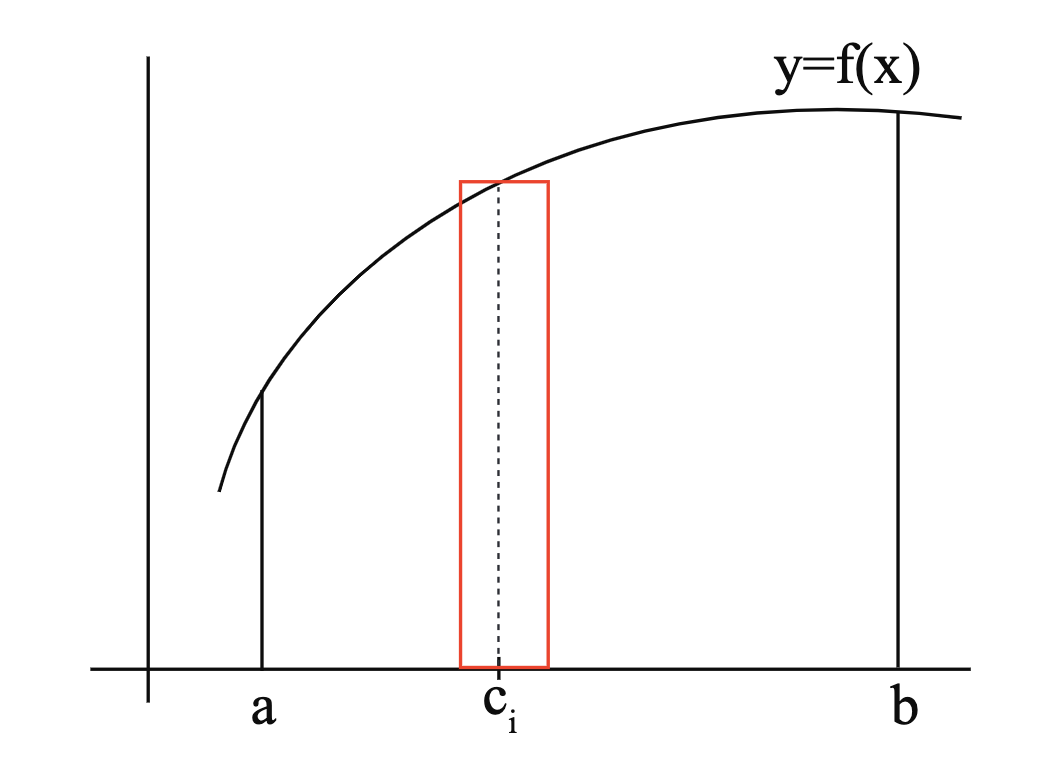
\includegraphics[scale=0.5]{./images/lecture_12_figure_2.png}
	\caption{One Rectangle from a Riemann Sum}
\end{figure}

\begin{itemize}
	\item Divide into $n$ equal pieces of length \ilds{ = \Delta x = \frac{b-a}{n} }
	\item Pick any $c_i$ in the interaval; use $f(c_i)$ as the height of the rectangle
	\item Sum of areas : $f(c_1)\Delta x + f(c_2)\Delta x + \cdots + f(c_n)\Delta x$
\end{itemize}

In summation notation: \ilds{ \sum^n_{i=1} f(c_i)\Delta x \longleftarrow } called a {\it Riemann Sum}.

\subsubsection{Definition:}
$$
\lim_{n \to \infty} \sum^n_{i=1} f(c_i)\Delta x = \int_a^b f(x)dx \quad \leftarrow \text{ called a {\it Definition Integral}}
$$

This integral represents the area under the curve $y = f(x)$ above $[a, b]$.
